\documentclass{standalone}
\usepackage{tikz}
\usetikzlibrary{patterns, positioning}

\begin{document}
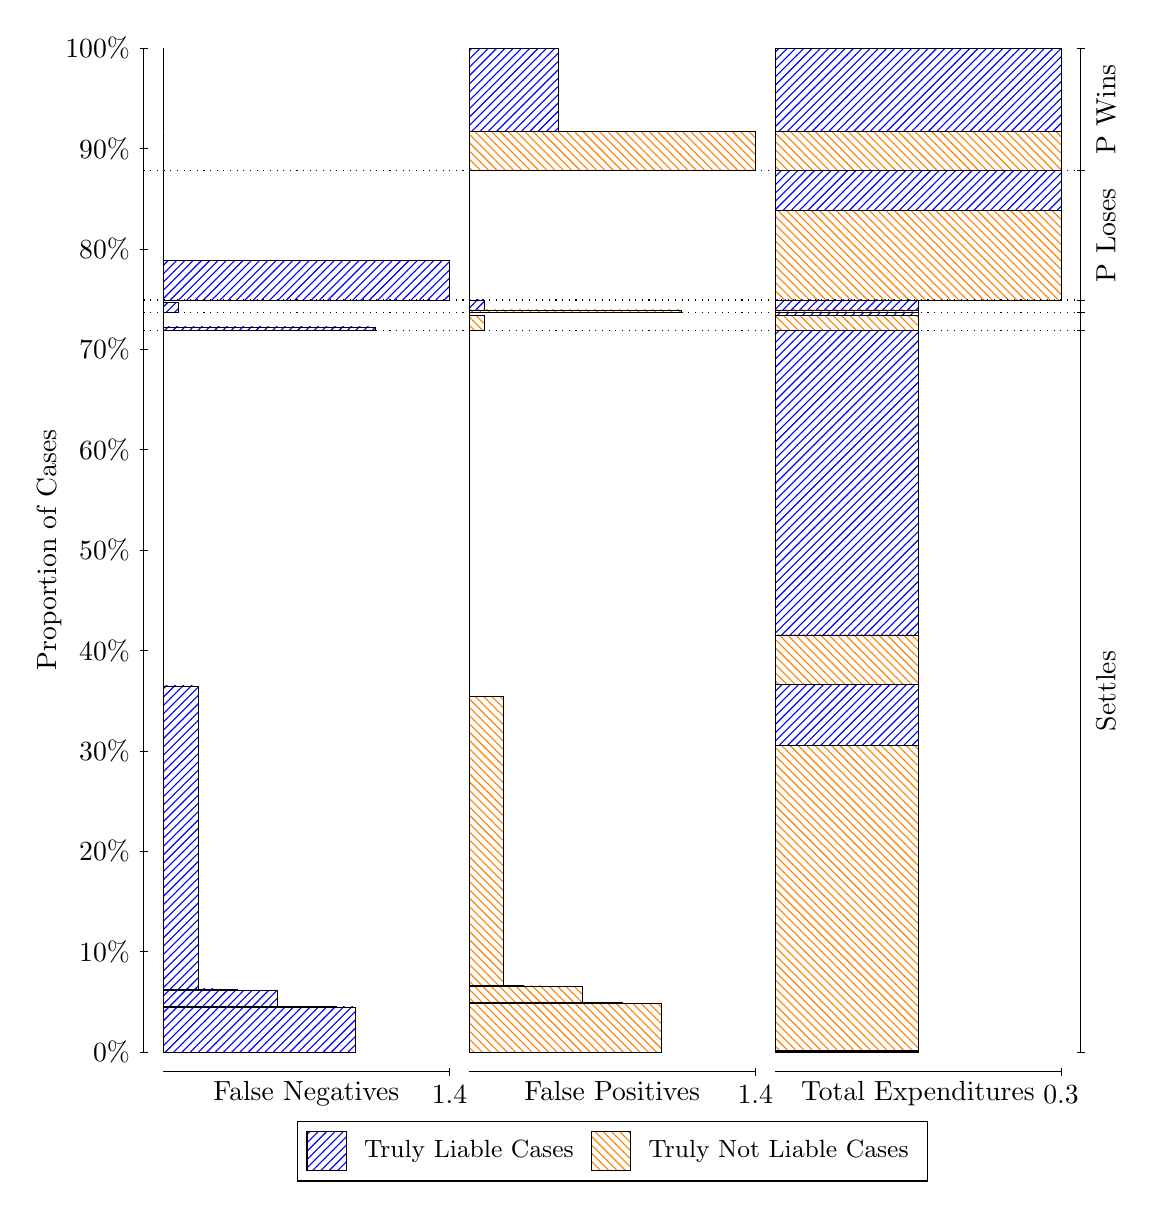
\begin{tikzpicture}
\draw[black, very thin] (1.5,1.75) -- (1.5,14.5);
\node[rotate=90, anchor=center] at (0.3, 8.125) {Proportion of Cases};
\draw[black, very thin] (1.45,1.75) -- (1.55,1.75);
\node[anchor=east] at (1.45, 1.75) {0\%};
\draw[black, very thin] (1.45,3.025) -- (1.55,3.025);
\node[anchor=east] at (1.45, 3.025) {10\%};
\draw[black, very thin] (1.45,4.3) -- (1.55,4.3);
\node[anchor=east] at (1.45, 4.3) {20\%};
\draw[black, very thin] (1.45,5.575) -- (1.55,5.575);
\node[anchor=east] at (1.45, 5.575) {30\%};
\draw[black, very thin] (1.45,6.85) -- (1.55,6.85);
\node[anchor=east] at (1.45, 6.85) {40\%};
\draw[black, very thin] (1.45,8.125) -- (1.55,8.125);
\node[anchor=east] at (1.45, 8.125) {50\%};
\draw[black, very thin] (1.45,9.4) -- (1.55,9.4);
\node[anchor=east] at (1.45, 9.4) {60\%};
\draw[black, very thin] (1.45,10.675) -- (1.55,10.675);
\node[anchor=east] at (1.45, 10.675) {70\%};
\draw[black, very thin] (1.45,11.95) -- (1.55,11.95);
\node[anchor=east] at (1.45, 11.95) {80\%};
\draw[black, very thin] (1.45,13.225) -- (1.55,13.225);
\node[anchor=east] at (1.45, 13.225) {90\%};
\draw[black, very thin] (1.45,14.5) -- (1.55,14.5);
\node[anchor=east] at (1.45, 14.5) {100\%};

\draw[black, very thin] (13.4,1.75) -- (13.4,14.5);
\draw[black, very thin] (13.35,1.75) -- (13.45,1.75);
\node[anchor=west] at (13.35, 1.75) {};
\draw[black, very thin] (13.35,10.916) -- (13.45,10.916);
\node[anchor=west] at (13.35, 10.916) {};
\draw[black, very thin] (13.35,11.145) -- (13.45,11.145);
\node[anchor=west] at (13.35, 11.145) {};
\draw[black, very thin] (13.35,11.3) -- (13.45,11.3);
\node[anchor=west] at (13.35, 11.3) {};
\draw[black, very thin] (13.35,12.943) -- (13.45,12.943);
\node[anchor=west] at (13.35, 12.943) {};
\draw[black, very thin] (13.35,14.5) -- (13.45,14.5);
\node[anchor=west] at (13.35, 14.5) {};

\draw[black, very thin, pattern color=blue, pattern=north east lines] (1.75,1.75) rectangle (4.1931,2.3226);
\draw[black, very thin, pattern color=blue, pattern=north east lines] (1.75,2.3226) rectangle (3.9425,2.3249);
\draw[black, very thin, pattern color=blue, pattern=north east lines] (1.75,2.3249) rectangle (3.692,2.3274);
\draw[black, very thin, pattern color=blue, pattern=north east lines] (1.75,2.3274) rectangle (3.4414,2.3298);
\draw[black, very thin, pattern color=blue, pattern=north east lines] (1.75,2.3298) rectangle (3.1908,2.5287);
\draw[black, very thin, pattern color=blue, pattern=north east lines] (1.75,2.5287) rectangle (2.9402,2.5357);
\draw[black, very thin, pattern color=blue, pattern=north east lines] (1.75,2.5357) rectangle (2.6897,2.5431);
\draw[black, very thin, pattern color=blue, pattern=north east lines] (1.75,2.5431) rectangle (2.4391,2.5506);
\draw[black, very thin, pattern color=blue, pattern=north east lines] (1.75,2.5506) rectangle (2.1885,6.3989);
\draw[black, very thin, pattern color=orange, pattern=north west lines] (1.75,6.3989) rectangle (1.75,10.916);
\draw[black, very thin, pattern color=blue, pattern=north east lines] (1.75,10.916) rectangle (4.4437,10.958);
\draw[black, very thin, pattern color=orange, pattern=north west lines] (1.75,10.958) rectangle (1.75,11.145);
\draw[black, very thin, pattern color=blue, pattern=north east lines] (1.75,11.145) rectangle (1.9379,11.271);
\draw[black, very thin, pattern color=orange, pattern=north west lines] (1.75,11.271) rectangle (1.75,11.3);
\draw[black, very thin, pattern color=blue, pattern=north east lines] (1.75,11.3) rectangle (5.3833,11.801);
\draw[black, very thin, pattern color=orange, pattern=north west lines] (1.75,11.801) rectangle (1.75,12.943);
\draw[black, very thin, pattern color=orange, pattern=north west lines] (1.75,12.943) rectangle (1.75,13.443);
\draw[black, very thin, pattern color=blue, pattern=north east lines] (1.75,13.443) rectangle (1.75,14.5);
\draw[black, very thin, pattern color=orange, pattern=north west lines] (5.6333,1.75) rectangle (8.0764,2.3638);
\draw[black, very thin, pattern color=orange, pattern=north west lines] (5.6333,2.3638) rectangle (7.8259,2.37);
\draw[black, very thin, pattern color=orange, pattern=north west lines] (5.6333,2.37) rectangle (7.5753,2.376);
\draw[black, very thin, pattern color=orange, pattern=north west lines] (5.6333,2.376) rectangle (7.3247,2.3818);
\draw[black, very thin, pattern color=orange, pattern=north west lines] (5.6333,2.3818) rectangle (7.0741,2.5837);
\draw[black, very thin, pattern color=orange, pattern=north west lines] (5.6333,2.5837) rectangle (6.8236,2.5838);
\draw[black, very thin, pattern color=orange, pattern=north west lines] (5.6333,2.5838) rectangle (6.8236,2.5867);
\draw[black, very thin, pattern color=orange, pattern=north west lines] (5.6333,2.5867) rectangle (6.573,2.5897);
\draw[black, very thin, pattern color=orange, pattern=north west lines] (5.6333,2.5897) rectangle (6.3224,2.5927);
\draw[black, very thin, pattern color=orange, pattern=north west lines] (5.6333,2.5927) rectangle (6.0718,6.2675);
\draw[black, very thin, pattern color=blue, pattern=north east lines] (5.6333,6.2675) rectangle (5.6333,10.916);
\draw[black, very thin, pattern color=orange, pattern=north west lines] (5.6333,10.916) rectangle (5.8213,11.103);
\draw[black, very thin, pattern color=blue, pattern=north east lines] (5.6333,11.103) rectangle (5.6333,11.145);
\draw[black, very thin, pattern color=orange, pattern=north west lines] (5.6333,11.145) rectangle (8.327,11.173);
\draw[black, very thin, pattern color=blue, pattern=north east lines] (5.6333,11.173) rectangle (5.8213,11.3);
\draw[black, very thin, pattern color=orange, pattern=north west lines] (5.6333,11.3) rectangle (5.6333,12.442);
\draw[black, very thin, pattern color=blue, pattern=north east lines] (5.6333,12.442) rectangle (5.6333,12.943);
\draw[black, very thin, pattern color=orange, pattern=north west lines] (5.6333,12.943) rectangle (9.2667,13.443);
\draw[black, very thin, pattern color=blue, pattern=north east lines] (5.6333,13.443) rectangle (6.7609,14.5);
\draw[black, very thin, pattern color=orange, pattern=north west lines] (9.5167,1.75) rectangle (11.333,1.759);
\draw[black, very thin, pattern color=blue, pattern=north east lines] (9.5167,1.759) rectangle (11.333,1.7663);
\draw[black, very thin, pattern color=orange, pattern=north west lines] (9.5167,1.7663) rectangle (11.333,5.6431);
\draw[black, very thin, pattern color=blue, pattern=north east lines] (9.5167,5.6431) rectangle (11.333,6.4145);
\draw[black, very thin, pattern color=orange, pattern=north west lines] (9.5167,6.4145) rectangle (11.333,7.0462);
\draw[black, very thin, pattern color=blue, pattern=north east lines] (9.5167,7.0462) rectangle (11.333,10.916);
\draw[black, very thin, pattern color=orange, pattern=north west lines] (9.5167,10.916) rectangle (11.333,11.103);
\draw[black, very thin, pattern color=blue, pattern=north east lines] (9.5167,11.103) rectangle (11.333,11.145);
\draw[black, very thin, pattern color=orange, pattern=north west lines] (9.5167,11.145) rectangle (11.333,11.173);
\draw[black, very thin, pattern color=blue, pattern=north east lines] (9.5167,11.173) rectangle (11.333,11.3);
\draw[black, very thin, pattern color=orange, pattern=north west lines] (9.5167,11.3) rectangle (13.15,12.442);
\draw[black, very thin, pattern color=blue, pattern=north east lines] (9.5167,12.442) rectangle (13.15,12.943);
\draw[black, very thin, pattern color=orange, pattern=north west lines] (9.5167,12.943) rectangle (13.15,13.443);
\draw[black, very thin, pattern color=blue, pattern=north east lines] (9.5167,13.443) rectangle (13.15,14.5);
\draw[black, dotted] (1.5,10.916) -- (13.4,10.916);
\draw[black, dotted] (1.5,11.145) -- (13.4,11.145);
\draw[black, dotted] (1.5,11.3) -- (13.4,11.3);
\draw[black, dotted] (1.5,12.943) -- (13.4,12.943);
\draw[black, very thin] (1.75,1.5) -- (5.3833,1.5);
\node[anchor=north] at (3.5667, 1.5) {False Negatives};
\draw[black, very thin] (5.3833,1.45) -- (5.3833,1.55);
\node[anchor=north] at (5.3833, 1.45) {1.4};

\draw[black, very thin] (5.6333,1.5) -- (9.2667,1.5);
\node[anchor=north] at (7.45, 1.5) {False Positives};
\draw[black, very thin] (9.2667,1.45) -- (9.2667,1.55);
\node[anchor=north] at (9.2667, 1.45) {1.4};

\draw[black, very thin] (9.5167,1.5) -- (13.15,1.5);
\node[anchor=north] at (11.333, 1.5) {Total Expenditures};
\draw[black, very thin] (13.15,1.45) -- (13.15,1.55);
\node[anchor=north] at (13.15, 1.45) {0.3};

\node[black, centered, rotate=90] at (13.72, 6.3332) {Settles};


\node[black, centered, rotate=90] at (13.72, 12.121) {P Loses};
\node[black, centered, rotate=90] at (13.72, 13.721) {P Wins};

\draw (7.449999999999999,1.5) node[draw=none] (baseCoordinate) {};
\begin{scope}[align=center]
        \matrix[scale=0.5, draw=black, below=0.5cm of baseCoordinate, nodes={draw}, column sep=0.1cm]{
            \node[rectangle, draw, minimum width=0.5cm, minimum height=0.5cm, pattern=north east lines, pattern color=blue] {}; &
            \node[draw=none, font=\small] (B) {Truly Liable Cases}; &
            \node[rectangle, draw, minimum width=0.5cm, minimum height=0.5cm, pattern=north west lines, pattern color=orange] {}; &
            \node[draw=none, font=\small] (B) {Truly Not Liable Cases}; \\
            };
\end{scope}

\end{tikzpicture}
\end{document}